\documentclass{article}
\usepackage{amsthm, amsmath, graphicx}
\usepackage[margin=1in]{geometry}
\begin{document}
    \noindent\textbf{CS 373 Homework 5}\hfill Anchu A. Lee\\
    \noindent\today\\\\
    \noindent\textbf{Question 1.10a} Construct NFA that recognizes the star of the language in Exercise 1.6b
        \begin{center}
            $\{w\mid w$ contains at least three 1s$\}$\\
            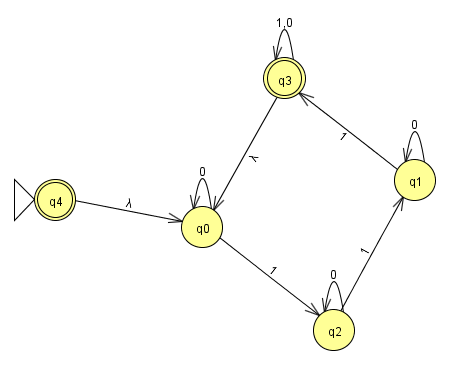
\includegraphics[scale=0.5]{q1}
        \end{center}
    \textbf{Question 1.10b} Same as before, but Exercise 1.6j
        \begin{center}
            $\{w\mid w $ contains at least two 0s and at most one 1$ \}$\\
            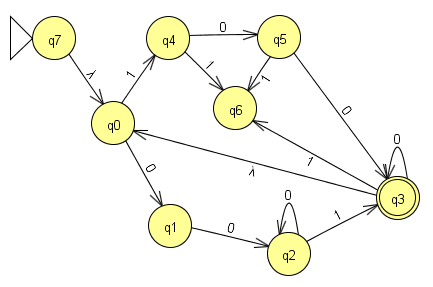
\includegraphics[scale=0.5]{q2}
        \end{center}
    \textbf{Question 1.29b} Use the pumping lemma to show that the language is not regular
        \begin{center}
            $A_2=\{www\mid w\in \{a,b\}^*\}$
        \end{center}
        \begin{proof}
            Assume $A_2$ is regular, then there must exist a number $n$ that is the pumping length. Test with the word $k = b^{n/2}b^{n/2}b^{n/2}$. $|k|>n$. Due to the nature of the language, there is only one way to split the word to satisfy the language. $x = b^{n/2}$; $y=b^{n/2}$; $z= b^{n/2}$. $|xy|\leq n$ and $|y|\geq 1$. Now consider pumping it up with $xy^iz$ for $i=2$. $xyz$ is not in $L$ because it is $b^{n/2}b^{n}b^{n/2}$ which does not match the definition of the language. Therefore our assumption was incorrect and $A_2$ is not regular.
        \end{proof}
    \textbf{Question 1.46a} Prove the following language is not regular using pumping lemma or closure of the class of regular languages under union, intersection, and compliment.
        \begin{center}
            $\{0^n1^m0^n\mid m,n \geq 0\}$
        \end{center}
        \begin{proof}
            Assume this language ($A$) is regular, so then it must be closed under compliment ($A'$). Then since regular languages are also closed under intersection, $(0^*1^*0^*)$ is regular so $A'\cap (0^*1^*0^*)$ should be as well. However that is not the case therefore our assumption that $A$ is regular was false.
        \end{proof}
    \textbf{Question 1.46c} Same as before
        \begin{center}
            $\{w\mid w\in \{0,1\}^* $ is not a palindrome$ \}$
        \end{center}
    \textbf{Question 1.46d} Same as before
        \begin{center}
            $\{wtw \mid w,t \in \{0.1\}^+ \}$
        \end{center}
    \textbf{Question 1.47} Let $\sum = \{1,\#\}$ and let 
        \begin{center}
            $Y=\{w\mid w=x_1\#x_2\#...\#x_k $ for $ k \geq 0 $, each $ x_i\in 1^* $, and $ x_i\not= x_j $ for $ i\not= j \}$
        \end{center}
    \textbf{Question 1.49}
        \begin{itemize}
            \item Let $B= \{1^ky\mid y\in \{0,1\}^*$ and $y$ contains at least $k$ 1s, for $k\geq 1\}$.\\
                  Show that $B$ is a regular language.
            \item Let $C= \{1^k y\mid y\in \{0,1\}^* $ and $y$ contains at most $k$ 1s, for $k\geq 1\}$.\\
                  Show that $C$ isn't a regular language.
        \end{itemize}
    \textbf{Show that $\{0^n1^m2^k\mid k$ divides $n+m\}$ is not regular.}\\
    \textbf{Convert the following NFA to a DFA}:\\
    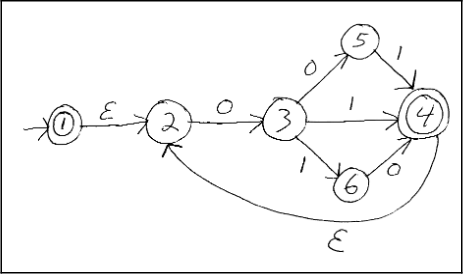
\includegraphics[scale=0.75]{machine}
\end{document}